\documentclass[11pt, a4paper]{MATH2023}
\usepackage{fancyhdr}
\usepackage{setspace}
\usepackage{amsmath,mathrsfs}
\usepackage{multicol}
\usepackage{amssymb}
\usepackage{graphicx}
\usepackage{caption}
\usepackage{subcaption}
\usepackage{xcolor}
\usepackage{enumitem}
\usepackage{tikz}
\usepackage{mathtools}
\usetikzlibrary{matrix}
\usepackage[normalem]{ulem}
\usepackage{multirow}
\usepackage[linesnumbered, ruled, boxed]{algorithm2e}
\SetKwRepeat{Do}{do}{while}
\newcommand{\eg}{\textbf{[Example.] }}
\newcommand{\sol}{\textbf{[Solution.] }}
\newcommand{\ii}{{\bf i}}
\newcommand{\jj}{{\bf j}}
\newcommand{\kk}{{\bf k}}
\newcommand{\rr}{{\bf r}}
\newcommand{\FF}{{\bf F}}
\renewcommand{\div}{{\rm div\ }}
\newcommand{\curl}{{\rm curl\ }}
\newcommand{\pt}{\partial}


\title{Chapter 15}
\subtitle{Vector Field}

\begin{document}
\begin{spacing}{1.3}

    \section{Intro. to Vector Field}

    So far, we have learned two kinds of functions involving vector: 
    \begin{itemize}
        \item ${\bf r}(t)=x(t){\bf i}+y(t){\bf j}+z(t){\bf k}$: for each $t$, provides a {\it position} vector 
        $<x(t), y(t), z(t)>$, so this is a (parametric) curve.
        \item $z=f({\bf r})=f(x_1,x_2,\cdots,x_n)$: for a given vector ${\rm r}$, this gives a real number,
        so this is a function of {\it several variables}. This is also a {\bf scalar field} since for 
        any point ${\bf r}$ in {\bf field}, it gives a scalar value. 
    \end{itemize}
    Now we are looking at {\bf vector-valued} function ${\bf F}$ of a vector ${\bf r}$, i.e., ${\bf F(r)}$.
    This is a {\bf vector field}, which means for any point ${\bf r}$ in {\bf field}, it gives a vector 
    ${\bf F(r)}$. 

    You can consider a world map showing the {\it speed} and {\it direction} of wind.
    \begin{center}
        \includegraphics[scale=0.17]{images/Ch15-wind.JPG}
    \end{center}

    You can see that in a 2D map(like above), if we put a vector on each point, the vector must have 
    same dimension as the map, i.e., all vectors must also be 2D vectors.
    $${\bf F(r)}=\left\{
        \begin{array}{lll}
            (F_1({\bf r}), F_2({\bf r})) & {\bf r}=(x,y) & {\blue 2D}\\
            (F_1({\bf r}), F_2({\bf r}), F_3({\bf r})) & {\bf r}=(x,y,z) & {\blue 3D}\\
            (F_1({\bf r}), F_2({\bf r}), \cdots, F_n({\bf r})) & {\bf r}=(x_1, x_2,\cdots, x_n) & {\blue nD}
        \end{array}\right.$$
    {\bf Summary:} {\it dimension of ${\bf F}$ must be the same as ${\bf r}$.}

    \eg Assume a vector field: ${\bf F}(x,y)=\dfrac{y\ii -x\jj}{\sqrt{x^2+y^2}}$.

    \sol Notice that $||{\bf F}||=\dfrac{y^2}{x^2+y^2}+\dfrac{x^2}{x^2+y^2}=1$, all vectors 
    ${\bf F}(x,y)$ are unit vectors. Moreover, let ${\bf r}=(x,y)$, then ${\bf r}\cdot {\bf F}=0$,
    so ${\bf r}\bot {\bf F}$.

    So all vectors are unit vectors tangent to circles centered at the origin with radius $\sqrt{x^2+y^2}$.
    \begin{center}
        \includegraphics[scale=0.4]{images/Ch15-ex1.2.png}
    \end{center}

    \newpage
    \section{Divergence and Curl}

    Recall that the {\bf gradient operator} is a {\it vector operator}:
    $$\nabla =\left(\frac{\pt}{\pt x}, \frac{\pt}{\pt y}, \frac{\pt}{\pt z}\right)\qquad {\blue \rm (a\ vector)}$$

    If $\FF (\rr)=F_1(\rr)\ii +F_2(\rr) \jj +F_3(\rr) \kk$, then we define: 
    \begin{itemize}
        \item {\bf divergence} of $\FF$, written $\div \FF$: 
        $$
        \operatorname{div} \mathbf{F}=\nabla \cdot \mathbf{F}=\frac{\partial F_1}{\partial x}+\frac{\partial F_2}{\partial y}+\frac{\partial F_3}{\partial z}
        $$
        \item {\bf curl} of $\FF$, written $\curl \FF$: 
        $$
        \operatorname{curl} \mathbf{F}=\nabla \times \mathbf{F}=\left|\begin{array}{ccc}
        \mathbf{i} & \mathbf{j} & \mathbf{k} \\
        \dfrac{\partial}{\partial x} & \dfrac{\partial}{\partial y} & \dfrac{\partial}{\partial z} \\
        F_1 & F_2 & F_3
        \end{array}\right|=\left(\frac{\partial h}{\partial y}-\frac{\partial g}{\partial z}\right) \mathbf{i}-\left(\frac{\partial h}{\partial x}-\frac{\partial f}{\partial z}\right) \mathbf{j}+\left(\frac{\partial g}{\partial x}-\frac{\partial f}{\partial y}\right) \mathbf{k}
        $$
    \end{itemize}

    \vspace{0.2in}
    {\blue This example shows basic computation of {\bf divergence} and {\bf curl}.}

    \eg Let $\mathbf{r}=x \mathbf{i}+y \mathbf{j}+z \mathbf{k}$ and $\mathbf{u}=a \mathbf{i}+b \mathbf{j}+c \mathbf{k}$, where $a, b$ and $c$ are constants, show that

    (a) $\nabla \cdot \mathbf{r}=3$\\
    (b) $\nabla \times \mathbf{r}=\mathbf{0}$\\
    (c) $\nabla \cdot(\mathbf{u} \times \mathbf{r})=0$\\
    (d) $\nabla \times(\mathbf{u} \times \mathbf{r})=2 \mathbf{u}$.

    \sol 
    (a) $\disp \nabla \cdot \mathbf{r}=\left(\mathbf{i} \frac{\partial}{\partial x}+\mathbf{j} \frac{\partial}{\partial y}+\mathbf{k} \frac{\partial}{\partial z}\right) \cdot(x \mathbf{i}+y \mathbf{j}+z \mathbf{k})=
    \frac{\partial x}{\partial x}+\frac{\partial y}{\partial y}+\frac{\partial z}{\partial z}=3$

    (b) $\disp \nabla \times \mathbf{r}=\left|\begin{array}{ccc}
            \mathbf{i} & \mathbf{j} & \mathbf{k} \\ 
            \frac{\partial}{\partial x} & \frac{\partial}{\partial y} & \frac{\partial}{\partial z} \\ 
            x & y & z
        \end{array}\right|=\mathbf{0}$

    (c) $\disp \mathbf{u} \times \mathbf{r}=\left|\begin{array}{ccc}
            \mathbf{i} & \mathbf{j} & \mathbf{k} \\ 
            a & b & c \\ 
            x & y & z
        \end{array}\right|=(b z-c y) \mathbf{i}-(a z-c x) \mathbf{j}+(a y-b x) \mathbf{k}$

    $\disp \therefore \nabla \cdot(\mathbf{u} \times \mathbf{r})=\frac{\partial}{\partial x}(b z-c y)-\frac{\partial}{\partial y}(a z-c x)+\frac{\partial}{\partial z}(a y-b x)=0$

    (d) $\disp \nabla \times(\mathbf{u} \times \mathbf{r})=\left|\begin{array}{ccc}\mathbf{i} & \mathbf{j} & \mathbf{k} \\ \frac{\partial}{\partial x} & \frac{\partial}{\partial y} & \frac{\partial}{\partial z} \\ b z-c y & -a z+c x & a y-b x\end{array}\right|=2(a \mathbf{i}+b \mathbf{j}+c \mathbf{k})=2 \mathbf{u}$


    \newpage
    \subsection{Interpretation of Divergence}

    \newcommand{\uu}{{\bf u}}

    Imagine water in a bath tank, if the {\bf velocity} of water at any point 
    of the tank is given by $$\uu (\rr)=u_1(\rr) \ii +u_2(\rr) \jj + u_3(\rr)\kk$$
    then {\bf net outward flux per unit volume} is $\div \uu =\nabla \cdot \uu$.
    \begin{center}
        \includegraphics[scale=0.18]{images/Ch15-bath.JPG}
    \end{center}
    Moreover, 
    \begin{itemize}
        \item If more water comes inside, then $\div \uu <0$
        \item If more water comes outside, then $\div \uu >0$
        \item If the amount of water comes inside equals to comes outside, then $\div \uu =0$
    \end{itemize}

    \newpage
    {\blue This page proves the interpretation of divergence.}
    \begin{center}
    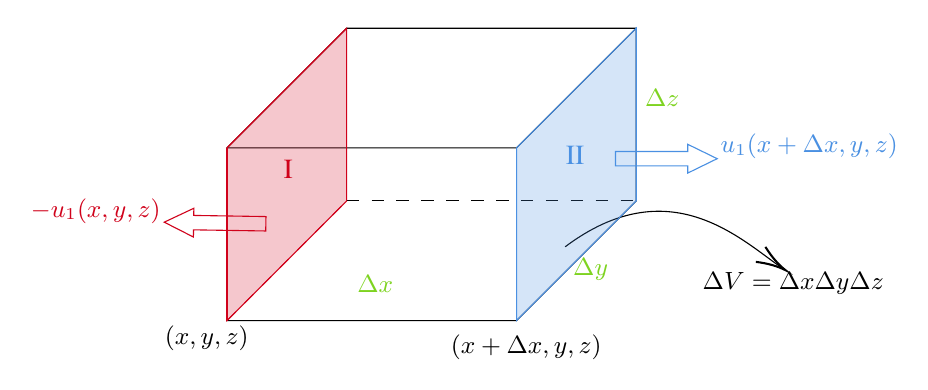
\begin{tikzpicture}[x=0.75pt,y=0.75pt,yscale=-1,xscale=1,scale=1.3]
    %uncomment if require: \path (0,155); %set diagram left start at 0, and has height of 155

    %Shape: Cube [id:dp6186431636735903] 
    \draw   (119.33,59.35) -- (163.68,15) -- (271,15) -- (271,79) -- (226.65,123.35) -- (119.33,123.35) -- cycle ; \draw   (271,15) -- (226.65,59.35) -- (119.33,59.35) ; \draw   (226.65,59.35) -- (226.65,123.35) ;
    %Straight Lines [id:da26318241804807796] 
    \draw [color={rgb, 255:red, 208; green, 2; blue, 27 }  ,draw opacity=1 ] [dash pattern={on 4.5pt off 4.5pt}]  (163.68,15) -- (163.68,79) ;
    %Straight Lines [id:da5928581432545683] 
    \draw  [dash pattern={on 4.5pt off 4.5pt}]  (163.67,79) -- (271,79) ;
    %Straight Lines [id:da8393161561837947] 
    \draw [color={rgb, 255:red, 208; green, 2; blue, 27 }  ,draw opacity=1 ] [dash pattern={on 4.5pt off 4.5pt}]  (119.33,123.35) -- (163.68,79) ;
    %Straight Lines [id:da08992921676399823] 
    \draw [color={rgb, 255:red, 208; green, 2; blue, 27 }  ,draw opacity=1 ]   (119.33,59.35) -- (163.68,15) ;
    %Straight Lines [id:da893341395756176] 
    \draw [color={rgb, 255:red, 208; green, 2; blue, 27 }  ,draw opacity=1 ]   (119.33,59.35) -- (119.33,123.35) ;
    %Curve Lines [id:da8206306595575221] 
    \draw    (244.67,96) .. controls (283.27,67.05) and (309.76,93.37) .. (324.75,103.63) ;
    \draw [shift={(326.33,104.68)}, rotate = 212.47] [color={rgb, 255:red, 0; green, 0; blue, 0 }  ][line width=0.75]    (10.93,-3.29) .. controls (6.95,-1.4) and (3.31,-0.3) .. (0,0) .. controls (3.31,0.3) and (6.95,1.4) .. (10.93,3.29)   ;
    %Shape: Polygon [id:ds9782874362859937] 
    \draw  [color={rgb, 255:red, 208; green, 2; blue, 27 }  ,draw opacity=1 ][fill={rgb, 255:red, 208; green, 2; blue, 27 }  ,fill opacity=0.22 ] (119.33,59.35) -- (146.83,31.85) -- (163.68,15) -- (163.68,79) -- (119.33,123.35) -- cycle ;
    %Shape: Polygon [id:ds6319731068332441] 
    \draw  [color={rgb, 255:red, 74; green, 144; blue, 226 }  ,draw opacity=1 ][fill={rgb, 255:red, 74; green, 144; blue, 226 }  ,fill opacity=0.23 ] (271,15) -- (271,79) -- (226.65,123.35) -- (226.65,59.35) -- cycle ;
    %Right Arrow [id:dp006127051123159699] 
    \draw  [color={rgb, 255:red, 74; green, 144; blue, 226 }  ,draw opacity=1 ] (263.33,60.68) -- (290.1,60.68) -- (290.1,58.02) -- (301,63.35) -- (290.1,68.68) -- (290.1,66.02) -- (263.33,66.02) -- cycle ;
    %Right Arrow [id:dp9412315249643457] 
    \draw  [color={rgb, 255:red, 208; green, 2; blue, 27 }  ,draw opacity=1 ] (133.69,90.14) -- (106.93,89.72) -- (106.89,92.38) -- (96.07,86.88) -- (107.05,81.72) -- (107.01,84.38) -- (133.78,84.8) -- cycle ;

    % Text Node
    \draw (139.33,63) node [anchor=north west][inner sep=0.75pt]  [color={rgb, 255:red, 208; green, 2; blue, 27 }  ,opacity=1 ] [align=left] {{\fontfamily{ptm}\selectfont I}};
    % Text Node
    \draw (244,57.67) node [anchor=north west][inner sep=0.75pt]  [color={rgb, 255:red, 74; green, 144; blue, 226 }  ,opacity=1 ] [align=left] {{\fontfamily{ptm}\selectfont II}};
    % Text Node
    \draw (95.33,124.4) node [anchor=north west][inner sep=0.75pt]  [font=\small]  {$( x,y,z)$};
    % Text Node
    \draw (201.33,127.73) node [anchor=north west][inner sep=0.75pt]  [font=\small]  {$( x+\Delta x,y,z)$};
    % Text Node
    \draw (166.67,105.73) node [anchor=north west][inner sep=0.75pt]  [font=\small,color={rgb, 255:red, 126; green, 211; blue, 33 }  ,opacity=1 ]  {$\Delta x$};
    % Text Node
    \draw (246.67,99.4) node [anchor=north west][inner sep=0.75pt]  [font=\small,color={rgb, 255:red, 126; green, 211; blue, 33 }  ,opacity=1 ]  {$\Delta y$};
    % Text Node
    \draw (273.33,36.73) node [anchor=north west][inner sep=0.75pt]  [font=\small,color={rgb, 255:red, 126; green, 211; blue, 33 }  ,opacity=1 ]  {$\Delta z$};
    % Text Node
    \draw (294.67,104.73) node [anchor=north west][inner sep=0.75pt]  [font=\small]  {$\Delta V=\Delta x\Delta y\Delta z$};
    % Text Node
    \draw (301.33,53.07) node [anchor=north west][inner sep=0.75pt]  [font=\small,color={rgb, 255:red, 74; green, 144; blue, 226 }  ,opacity=1 ]  {$u_{1}( x+\Delta x,y,z)$};
    % Text Node
    \draw (45.67,77.07) node [anchor=north west][inner sep=0.75pt]  [font=\small,color={rgb, 255:red, 208; green, 2; blue, 27 }  ,opacity=1 ]  {$-u_{1}( x,y,z)$};

    \end{tikzpicture}
    \end{center}

    Imagine the box with volume $\Delta V=\Delta x\Delta y\Delta z$, firstly consider faces $\rm \red I$ and $\rm \blue II$,
    the total flux {\it out of} faces $\rm \red I$ and $\rm \blue II$, as shown above, is: 
    \begin{align*}
        & [{\blue u_1(x+\Delta x,y,z)}-{\red u_1(x,y,z)}] \Delta y \Delta z\\
        = & \frac{[{\blue u_1(x+\Delta x,y,z)}-{\red u_1(x,y,z)}]}{\Delta x} \Delta x \Delta y \Delta z\\
        = & \frac{\pt u_1}{\pt x} \Delta x \Delta y \Delta z, \qquad {\rm( in\ the\ limit\ of\ } \Delta x\rightarrow 0)
    \end{align*}

    Similarly, the two faces in the $y-$ and $z-$ direction contribute 
    $$\frac{\pt u_2}{\pt y} \Delta x \Delta y \Delta z, \quad \frac{\pt u_3}{\pt z} \Delta x \Delta y \Delta z$$

    Hence net outward flux is: 
    $$\left(\frac{\pt u_1}{\pt x} + \frac{\pt u_2}{\pt y} + \frac{\pt u_3}{\pt z}\right)\cdot \Delta V$$
    Therefore outward flux {\it per unit volume} is $\nabla \cdot \uu$.



    \newpage
    \subsection{Interpretation of Curl}

    Curl is something related to rotation. Consider a small object flying in strong wind,
    the speed and direction of wind can be treated as a vector field, and 
\end{spacing}
\end{document}
